% !TeX root = ../main.tex
% LLD: Low Level Design

\chapter{详细设计与实现}

本章节主要在概要设计的基础之上, 对本中文时间表达式信息抽取系统的详细设计给出具体解决方案并进行实现, 其内容主要包括各个模块的详细设计和逻辑实现.
本章节深入理解概率无关上下文语法的原理及其工作的上下文环境, 设计实现各种识别和解析规则, 完成本中文时间表达式信息抽取系统的编码实现.


\section{中文时间表达式识别模块的设计与实现}

\subsection{概述}

中文时间表达式的识别和解析都是以概率无关上下文语法为核心算法实现的.
对于中文时间表达式, 涉及到两个比较关键的部分, 一部分是对数字部分的识别, 另一部分是对时间单元的识别, 最后是有机的将这些识别规则组合到一起.
概率无关上下文语法通常四元组的形式出现: (N, R, S,  $\varSigma$). 其中N代表的是非终止符号集合, $\varSigma$ 代表的是终止符号的集合, $\varSigma$.
R代表的是一规则或者是产生式的结合, 对于每一个产生式, 其组成形式应该为 A $\rightarrow$ $\beta$[p], 其中A应该为一个非终止符, beta是一个包含0个或多个符号的字符串,
字符串的形式应该为($\varSigma$ $\cup$ N), 即非终结符与终结符的交集中产生的字符串. p则为一个介于0和1中间的数字, 表示 P($\beta$|A)的概率.
P($\beta$|A)可以理解为由终止符产生相应的表达式字符串的概率, 即该产生式的概率.
S则为起始符号.


\subsection{数值类型识别子模块的设计与实现}

\subsubsection{数值类型终止符定义}

数值类型终止符主要涉及到阿拉伯数字与中文数字的识别, 出于使用场景的考虑, 文字识别中并没有带上英文数字表示, 那已经超过日常生产环境的使用范围.

数值类型终止符主要通过

\begin{table}[h]
    \centering
    \caption{部分数值类型终止符}
    \begin{tabular}{*{4}{c}}
        \toprule
        类名                  & 描述                                                                         & 蕴含字符                       & 对应数字                          \\
        \midrule
        CHINESE\_DIGITS       & 简体中文数字                                                                 & \makecell*[c]{〇,一, 二,三,四,                                     \\ 五,六,七,八,九} & \makecell*[c]{0, 1, 2, 3, 4, \\ 5, 6, 7, 8, 9}         \\
        CHINESE\_DIGITS\_TRAD & 繁体中文数字                                                                 & \makecell*[c]{零,壹,贰,叁,肆,                                      \\ 伍,陆,柒,捌,玖}  & \makecell*[c]{0, 1, 2, 3, 4, \\ 5, 6, 7, 8, 9}         \\
        CHINESE\_UNITS        & \makecell*[c]{简体中文                                             数字单位} & \makecell*[c]{十, 百, 千,                                          \\ 万, 十万, 百万}     & \makecell*[c]{$10^1, 10^2, 10^3,$ \\ $10^4, 10^5, 10^6$} \\
        CHINESE\_UNITS\_TRAD  & \makecell*[c]{繁体中文                                             数字单位} & 拾,佰,仟,萬,億                 & \makecell*[c]{$10^1, 10^2, 10^3,$ \\ $10^4, 10^8$}       \\
        ARABIC\_DIGIT         & 阿拉伯数字                                                                   & \makecell*[c]{0, 1, 2, 3, 4,                                       \\ 5, 6, 7, 8, 9} & \makecell*[c]{0, 1, 2, 3, 4, \\ 5, 6, 7, 8, 9}         \\
        MIXED\_SIGNS          & 正负符号                                                                     & 正, +, 负, -                   & 1, 1, -1, -1                      \\
        \bottomrule
    \end{tabular}
\end{table}


\begin{figure}[h]
    \centering
    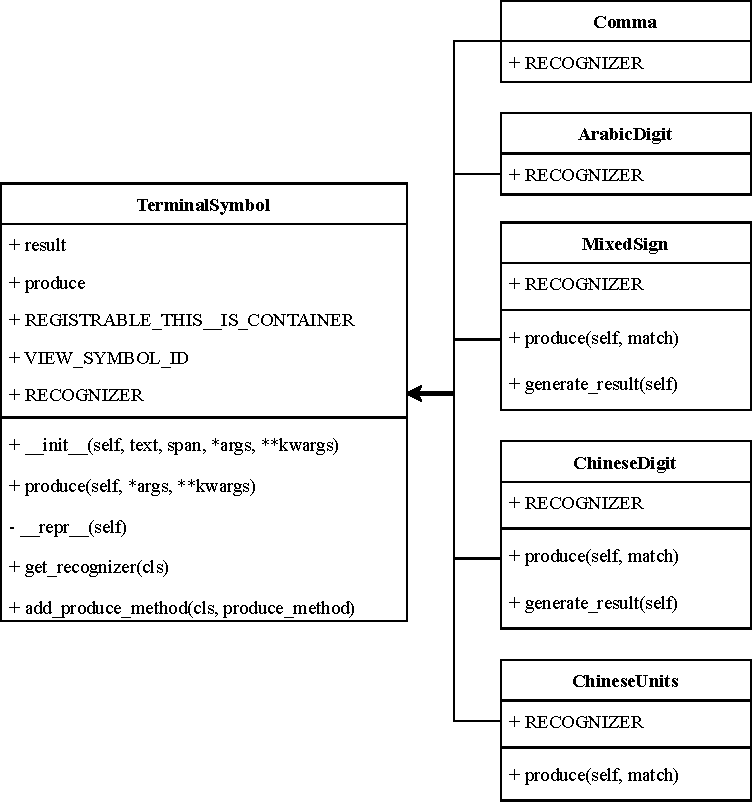
\includegraphics[width=1\textwidth]{numeral_terminal.pdf}
    \caption{数值类型终止符号类图}
    \label{fig:badge}
\end{figure}


其中部分与数值类型相关的终止符定义如下:



\begin{table}[h]
    \centering
    \caption{部分数值类型非终止符及产生式}
    \begin{tabular}{*{4}{c}}
        \toprule
        类名                               & 描述                   & 产生式                                                                                                                                         & 示例           \\
        \midrule
        \makecell*[c]{CHINESE \\ \_MIXED\_DIGITS \\ \_AND\_UNITS} & \makecell*[c]{中文阿拉伯\\数字混合类型} & \makecell*[c]{class \rightarrow MixedDigits + ChineseUnits; \\ class \rightarrow ArabicUnsignedInteger + ChineseUnits} & \makecell*[c]{3千4百\\八十六万} \\
        \bottomrule
    \end{tabular}
\end{table}

\begin{figure}[h]
    \centering
    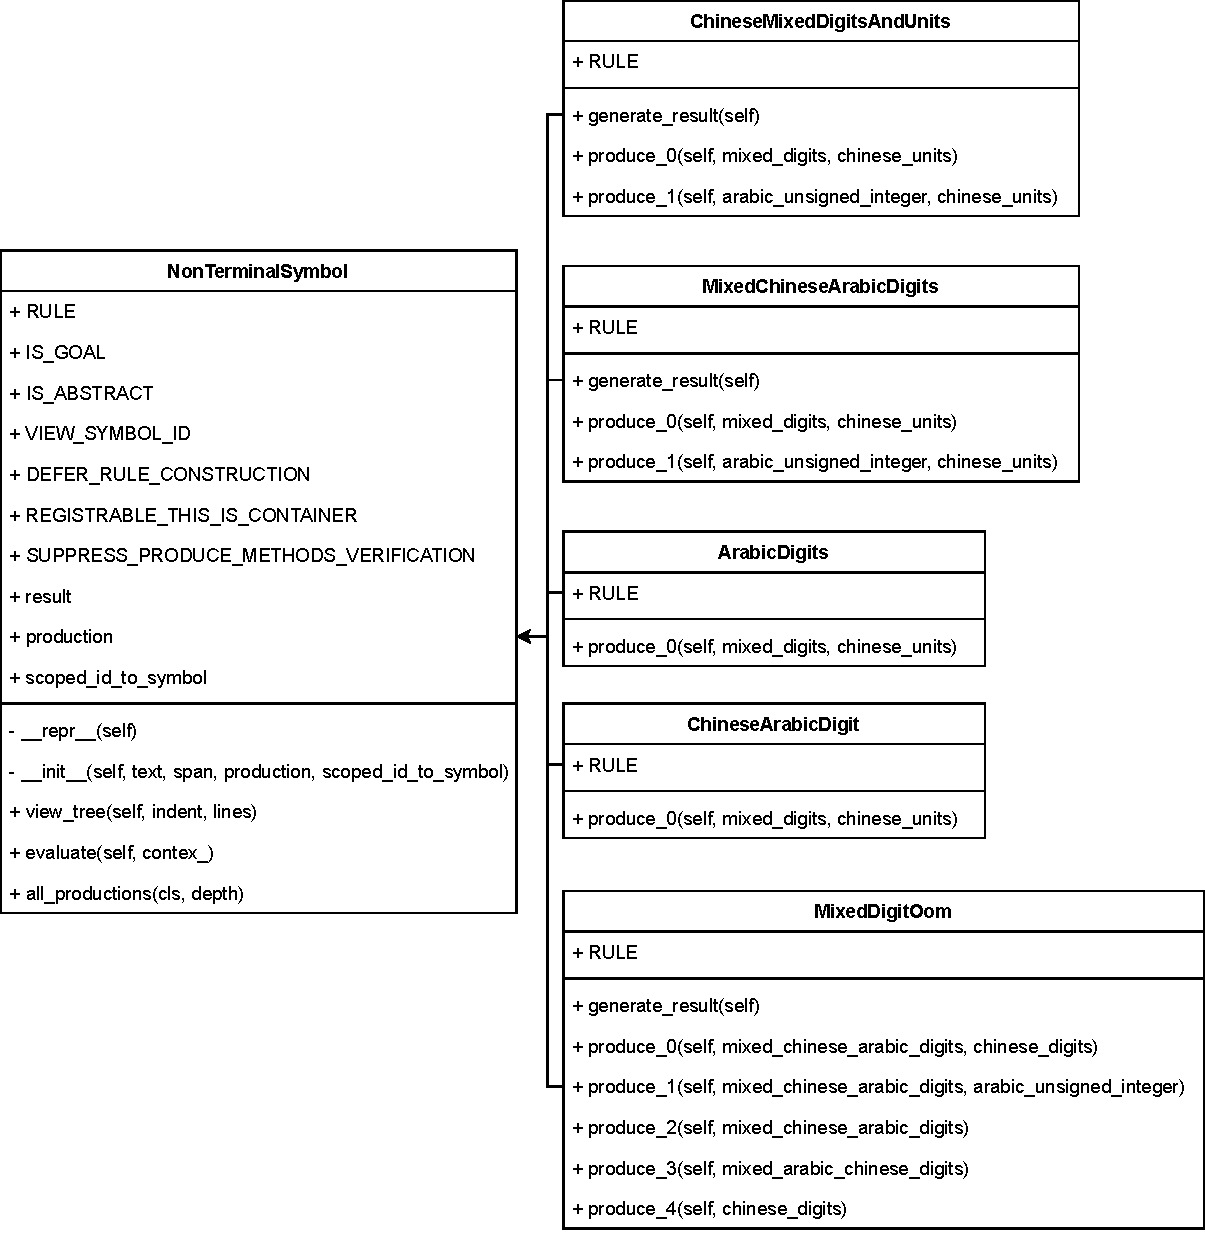
\includegraphics[width=1\textwidth]{numeral_nonterminal.pdf}
    \caption{部分数值类型非终止符号类图}
    \label{fig:badge}
\end{figure}


\subsubsection{预处理过程}

在前文中已经给出定义与时间表达式相关的终结符(terminal)和非终结符(non-terminals),终结
符在文本匹配中类似于正则表达式,以确定时间表达式的区间(span)。非终结符则在最后对
时间表达式抽象成的语法树中充当非叶结点。图 6 中由终结符和非终结符组成的产生式
(production)最终将被简化为 CNF(Chomsky norm function)。同时我们需要向语料库中写入
语料,语料库中的每条数据应该以(文本,结果)的文本对的形式存储,语料库作为训练集以
求得每个产生式的似然。产生式的似然将参与求得语法树整体概率的计算.
在前文中已经给出定义与时间表达式相关的终结符(terminal)和非终结符(non-terminals),终结
符在文本匹配中类似于正则表达式,以确定时间表达式的区间(span)。非终结符则在最后对
时间表达式抽象成的语法树中充当非叶结点。图 6 中由终结符和非终结符组成的产生式
(production)最终将被简化为 CNF(Chomsky norm function)。同时我们需要向语料库中写入
语料,语料库中的每条数据应该以(文本,结果)的文本对的形式存储,语料库作为训练集以
求得每个产生式的似然。产生式的似然将参与求得语法树整体概率的计算.
在前文中已经给出定义与时间表达式相关的终结符(terminal)和非终结符(non-terminals),终结
符在文本匹配中类似于正则表达式,以确定时间表达式的区间(span)。非终结符则在最后对
时间表达式抽象成的语法树中充当非叶结点。图 6 中由终结符和非终结符组成的产生式
(production)最终将被简化为 CNF(Chomsky norm function)。同时我们需要向语料库中写入
语料,语料库中的每条数据应该以(文本,结果)的文本对的形式存储,语料库作为训练集以
求得每个产生式的似然。产生式的似然将参与求得语法树整体概率的计算.

\subsubsection{分析树的构建}

首先需要定义与时间表达式相关的终结符(terminal)和非终结符(non-terminals),终结
符在文本匹配中类似于正则表达式,以确定时间表达式的区间(span)。非终结符则在最后对
时间表达式抽象成的语法树中充当非叶结点。图 6 中由终结符和非终结符组成的产生式
(production)最终将被简化为 CNF(Chomsky norm function)。同时我们需要向语料库中写入
语料,语料库中的每条数据应该以(文本,结果)的文本对的形式存储,语料库作为训练集以
求得每个产生式的似然。产生式的似然将参与求得语法树整体概率的计算
首先需要定义与时间表达式相关的终结符(terminal)和非终结符(non-terminals),终结
符在文本匹配中类似于正则表达式,以确定时间表达式的区间(span)。非终结符则在最后对
时间表达式抽象成的语法树中充当非叶结点。图 6 中由终结符和非终结符组成的产生式
(production)最终将被简化为 CNF(Chomsky norm function)。同时我们需要向语料库中写入
语料,语料库中的每条数据应该以(文本,结果)的文本对的形式存储,语料库作为训练集以
求得每个产生式的似然。产生式的似然将参与求得语法树整体概率的计算
首先需要定义与时间表达式相关的终结符(terminal)和非终结符(non-terminals),终结
符在文本匹配中类似于正则表达式,以确定时间表达式的区间(span)。非终结符则在最后对
时间表达式抽象成的语法树中充当非叶结点。图 6 中由终结符和非终结符组成的产生式
(production)最终将被简化为 CNF(Chomsky norm function)。同时我们需要向语料库中写入
语料,语料库中的每条数据应该以(文本,结果)的文本对的形式存储,语料库作为训练集以
求得每个产生式的似然。产生式的似然将参与求得语法树整体概率的计算

\subsubsection{冲突消解}

\begin{figure}[h]
    \centering
    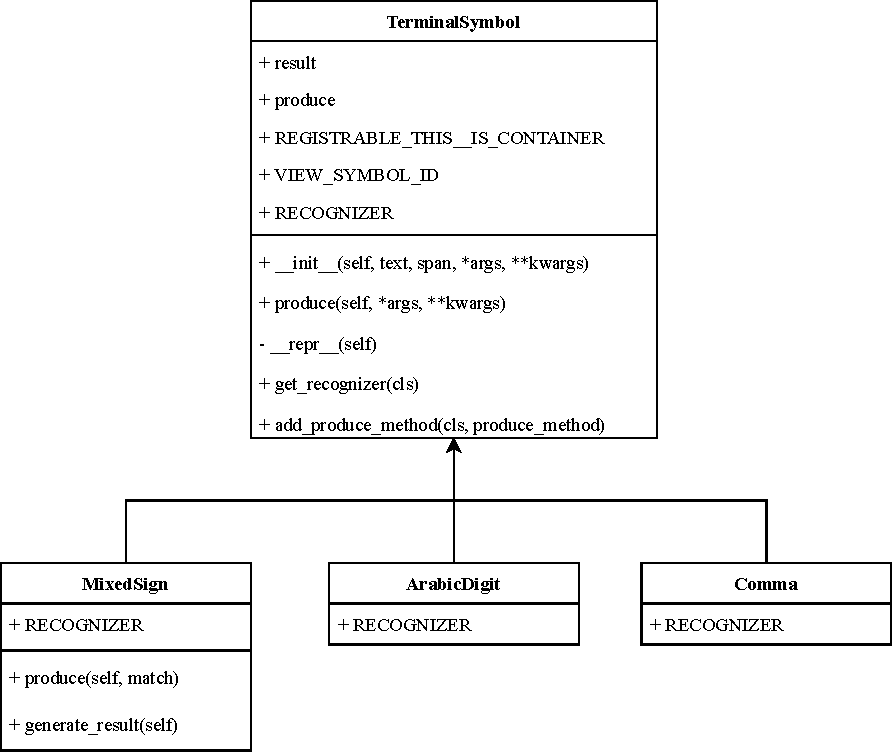
\includegraphics[width=1\textwidth]{arabic.pdf}
    \caption{系统功能模块图}
    \label{fig:badge}
\end{figure}

如图 9,同一个时间表达式可能解析出多棵语法树,需要最终选择在总概率上为 top-k 的
k 棵语法树,即总体概率最大的 k 棵树。解析树的整体概率为树上所有产生式概率的乘积,在
本项目中将 k 的值设为 1,则最终的语法树的概率如下。S 表示识别到的时间表达式,Tree 为
生成的解析树,n 为树中产生式的数量。


\subsection{中文时间表达式解析模块的设计与实现}

在使用句法分析获得时间表达式的语法树后,我们还需要将整棵树归一化到一种具体的
标注格式,这里我们选择了 SCATE 并加以改良,使其更贴合与中文的时间表达。归一化核心
的数据结构有三:
1) Period:时间轴上的基本时间单位数量之和,如‘3 天’,‘2 个小时 30 分钟’;
2) Interval:时间轴上一段左闭右开的,能确定到年份(year)的区间,如‘2019 年’,
‘2019 年 3 月’;
3) Repeat-interval:时间轴上一段左闭右开的,不包括年份,表示在时间轴上具有重复性
的一段区间,如‘3 月份’,‘5 点 20 分’。
我们以三种数据结构为核心,并用操作符集合(operator set)来表示时间表达式的语义。
在表 4 中列举出部分典型操作符。在构建时间表达式分析树的过程中,其实已经将操作符与数
据结构相结合,分析树构建完成后,树的根结点会将操作符集合形成嵌套表达式保存,直到我
们需要将时间表达式转化为特定的结构化信息时,才进行嵌套表达式的计算,以实现惰性计算
(lazy evaluation)。根结点的最终计算结果应该是以 ISO 格式描述的有起止时间的区间或类似
格式的时间段,如‘2019 年 3 月 2 日’,表达式最终计算的结果应该为‘Interval(start=2019-03-
02T00:00:00, end=2019-03-03T00:00:00)’。
在使用句法分析获得时间表达式的语法树后,我们还需要将整棵树归一化到一种具体的
标注格式,这里我们选择了 SCATE 并加以改良,使其更贴合与中文的时间表达。归一化核心
的数据结构有三:
1) Period:时间轴上的基本时间单位数量之和,如‘3 天’,‘2 个小时 30 分钟’;
2) Interval:时间轴上一段左闭右开的,能确定到年份(year)的区间,如‘2019 年’,
‘2019 年 3 月’;
3) Repeat-interval:时间轴上一段左闭右开的,不包括年份,表示在时间轴上具有重复性
的一段区间,如‘3 月份’,‘5 点 20 分’。
我们以三种数据结构为核心,并用操作符集合(operator set)来表示时间表达式的语义。
在表 4 中列举出部分典型操作符。在构建时间表达式分析树的过程中,其实已经将操作符与数
据结构相结合,分析树构建完成后,树的根结点会将操作符集合形成嵌套表达式保存,直到我
们需要将时间表达式转化为特定的结构化信息时,才进行嵌套表达式的计算,以实现惰性计算
(lazy evaluation)。根结点的最终计算结果应该是以 ISO 格式描述的有起止时间的区间或类似
格式的时间段,如‘2019 年 3 月 2 日’,表达式最终计算的结果应该为‘Interval(start=2019-03-
02T00:00:00, end=2019-03-03T00:00:00)’。
在使用句法分析获得时间表达式的语法树后,我们还需要将整棵树归一化到一种具体的
标注格式,这里我们选择了 SCATE 并加以改良,使其更贴合与中文的时间表达。归一化核心
的数据结构有三:
1) Period:时间轴上的基本时间单位数量之和,如‘3 天’,‘2 个小时 30 分钟’;
2) Interval:时间轴上一段左闭右开的,能确定到年份(year)的区间,如‘2019 年’,
‘2019 年 3 月’;
3) Repeat-interval:时间轴上一段左闭右开的,不包括年份,表示在时间轴上具有重复性
的一段区间,如‘3 月份’,‘5 点 20 分’。
我们以三种数据结构为核心,并用操作符集合(operator set)来表示时间表达式的语义。
在表 4 中列举出部分典型操作符。在构建时间表达式分析树的过程中,其实已经将操作符与数
据结构相结合,分析树构建完成后,树的根结点会将操作符集合形成嵌套表达式保存,直到我
们需要将时间表达式转化为特定的结构化信息时,才进行嵌套表达式的计算,以实现惰性计算
(lazy evaluation)。根结点的最终计算结果应该是以 ISO 格式描述的有起止时间的区间或类似
格式的时间段,如‘2019 年 3 月 2 日’,表达式最终计算的结果应该为‘Interval(start=2019-03-
02T00:00:00, end=2019-03-03T00:00:00)’。

\subsection{时间信息抽取系统分析与展示模块}

\subsubsection{用户前端交互模块设计}

中文时间表达式的识别和解析都是以概率无关上下文语法为核心算法实现的.
对于中文时间表达式, 涉及到两个比较关键的部分, 一部分是对数字部分的识别, 另一部分是对时间单元的识别, 最后是有机的将这些识别规则组合到一起.
概率无关上下文语法通常四元组的形式出现: (N, R, S,  $\varSigma$). 其中N代表的是非终止符号集合, $\varSigma$ 代表的是终止符号的集合, $\varSigma$.
R代表的是一规则或者是产生式的结合, 对于每一个产生式, 其组成形式应该为 A $\rightarrow$ $\beta$[p], 其中A应该为一个非终止符, beta是一个包含0个或多个符号的字符串,
字符串的形式应该为($\varSigma$ $\cup$ N), 即非终结符与终结符的交集中产生的字符串. p则为一个介于0和1中间的数字, 表示 P($\beta$|A)的概率.
P($\beta$|A)可以理解为由终止符产生相应的表达式字符串的概率, 即该产生式的概率.
S则为其实符号.

其中部分与中文整数相关的终止符定义如下:

\begin{table}[h]
    \centering
    \caption{部分中文整数终止符}
    \begin{tabular}{*{4}{c}}
        \toprule
        类名                  & 描述                                                                         & 蕴含字符                       & 对应数字                          \\
        \midrule
        CHINESE\_DIGITS       & 简体中文数字                                                                 & \makecell*[c]{〇,一, 二,三,四,                                     \\ 五,六,七,八,九} & \makecell*[c]{0, 1, 2, 3, 4, \\ 5, 6, 7, 8, 9}         \\
        CHINESE\_DIGITS\_TRAD & 繁体中文数字                                                                 & \makecell*[c]{零,壹,贰,叁,肆,                                      \\ 伍,陆,柒,捌,玖}  & \makecell*[c]{0, 1, 2, 3, 4, \\ 5, 6, 7, 8, 9}         \\
        CHINESE\_UNITS        & \makecell*[c]{简体中文                                             数字单位} & \makecell*[c]{十, 百, 千,                                          \\ 万, 十万, 百万}     & \makecell*[c]{$10^1, 10^2, 10^3,$ \\ $10^4, 10^5, 10^6$} \\
        CHINESE\_UNITS\_TRAD  & \makecell*[c]{繁体中文                                             数字单位} & 拾,佰,仟,萬,億                 & \makecell*[c]{$10^1, 10^2, 10^3,$ \\ $10^4, 10^8$}       \\
        \bottomrule
    \end{tabular}
\end{table}


部分与阿拉伯整数相关的终止符相关的终止符定义如下

\begin{table}[h]
    \centering
    \caption{部分中文整数终止符}
    \begin{tabular}{*{4}{c}}
        \toprule
        类名         & 描述       & 蕴含字符                     & 对应数字     \\
        \midrule
        ArabicDigit  & 阿拉伯数字 & \makecell*[c]{0, 1, 2, 3, 4,                \\ 5, 6, 7, 8, 9} & \makecell*[c]{0, 1, 2, 3, 4, \\ 5, 6, 7, 8, 9}         \\
        MIXED\_SIGNS & 正负符号   & 正, +, 负, -                 & 1, 1, -1, -1 \\
        \bottomrule
    \end{tabular}
\end{table}

\subsubsection{MongoDB查询语言设计}

在前文已经给出定义与时间表达式相关的终结符(terminal)和非终结符(non-terminals),终结
符在文本匹配中类似于正则表达式,以确定时间表达式的区间(span)。非终结符则在最后对
时间表达式抽象成的语法树中充当非叶结点。图 6 中由终结符和非终结符组成的产生式
(production)最终将被简化为 CNF(Chomsky norm function)。同时我们需要向语料库中写入
语料,语料库中的每条数据应该以(文本,结果)的文本对的形式存储,语料库作为训练集以
求得每个产生式的似然。产生式的似然将参与求得语法树整体概率的计算.



首先需要定义与时间表达式相关的终结符(terminal)和非终结符(non-terminals),终结
符在文本匹配中类似于正则表达式,以确定时间表达式的区间(span)。非终结符则在最后对
时间表达式抽象成的语法树中充当非叶结点。图 6 中由终结符和非终结符组成的产生式
(production)最终将被简化为 CNF(Chomsky norm function)。同时我们需要向语料库中写入
语料,语料库中的每条数据应该以(文本,结果)的文本对的形式存储,语料库作为训练集以
求得每个产生式的似然。产生式的似然将参与求得语法树整体概率的计算
首先需要定义与时间表达式相关的终结符(terminal)和非终结符(non-terminals),终结
符在文本匹配中类似于正则表达式,以确定时间表达式的区间(span)。非终结符则在最后对
时间表达式抽象成的语法树中充当非叶结点。图 6 中由终结符和非终结符组成的产生式
(production)最终将被简化为 CNF(Chomsky norm function)。同时我们需要向语料库中写入
语料,语料库中的每条数据应该以(文本,结果)的文本对的形式存储,语料库作为训练集以
求得每个产生式的似然。产生式的似然将参与求得语法树整体概率的计算
首先需要定义与时间表达式相关的终结符(terminal)和非终结符(non-terminals),终结
符在文本匹配中类似于正则表达式,以确定时间表达式的区间(span)。非终结符则在最后对
时间表达式抽象成的语法树中充当非叶结点。图 6 中由终结符和非终结符组成的产生式
(production)最终将被简化为 CNF(Chomsky norm function)。同时我们需要向语料库中写入
语料,语料库中的每条数据应该以(文本,结果)的文本对的形式存储,语料库作为训练集以
求得每个产生式的似然。产生式的似然将参与求得语法树整体概率的计算



如图 9,同一个时间表达式可能解析出多棵语法树,需要最终选择在总概率上为 top-k 的
k 棵语法树,即总体概率最大的 k 棵树。解析树的整体概率为树上所有产生式概率的乘积,在
本项目中将 k 的值设为 1,则最终的语法树的概率如下。S 表示识别到的时间表达式,Tree 为
生成的解析树,n 为树中产生式的数量。


\subsection{时间信息抽取系统分析结果与语料存取模块}

在使用句法分析获得时间表达式的语法树后,我们还需要将整棵树归一化到一种具体的
标注格式,这里我们选择了 SCATE 并加以改良,使其更贴合与中文的时间表达。归一化核心
的数据结构有三:
1) Period:时间轴上的基本时间单位数量之和,如‘3 天’,‘2 个小时 30 分钟’;
2) Interval:时间轴上一段左闭右开的,能确定到年份(year)的区间,如‘2019 年’,
‘2019 年 3 月’;
3) Repeat-interval:时间轴上一段左闭右开的,不包括年份,表示在时间轴上具有重复性
的一段区间,如‘3 月份’,‘5 点 20 分’。
我们以三种数据结构为核心,并用操作符集合(operator set)来表示时间表达式的语义。
在表 4 中列举出部分典型操作符。在构建时间表达式分析树的过程中,其实已经将操作符与数
据结构相结合,分析树构建完成后,树的根结点会将操作符集合形成嵌套表达式保存,直到我
们需要将时间表达式转化为特定的结构化信息时,才进行嵌套表达式的计算,以实现惰性计算
(lazy evaluation)。根结点的最终计算结果应该是以 ISO 格式描述的有起止时间的区间或类似
格式的时间段,如‘2019 年 3 月 2 日’,表达式最终计算的结果应该为‘Interval(start=2019-03-
02T00:00:00, end=2019-03-03T00:00:00)’。

在使用句法分析获得时间表达式的语法树后,我们还需要将整棵树归一化到一种具体的
标注格式,这里我们选择了 SCATE 并加以改良,使其更贴合与中文的时间表达。归一化核心
的数据结构有三:
1) Period:时间轴上的基本时间单位数量之和,如‘3 天’,‘2 个小时 30 分钟’;
2) Interval:时间轴上一段左闭右开的,能确定到年份(year)的区间,如‘2019 年’,
‘2019 年 3 月’;
3) Repeat-interval:时间轴上一段左闭右开的,不包括年份,表示在时间轴上具有重复性
的一段区间,如‘3 月份’,‘5 点 20 分’。
我们以三种数据结构为核心,并用操作符集合(operator set)来表示时间表达式的语义。
在表 4 中列举出部分典型操作符。在构建时间表达式分析树的过程中,其实已经将操作符与数
据结构相结合,分析树构建完成后,树的根结点会将操作符集合形成嵌套表达式保存,直到我
们需要将时间表达式转化为特定的结构化信息时,才进行嵌套表达式的计算,以实现惰性计算
(lazy evaluation)。根结点的最终计算结果应该是以 ISO 格式描述的有起止时间的区间或类似
格式的时间段,如‘2019 年 3 月 2 日’,表达式最终计算的结果应该为‘Interval(start=2019-03-
02T00:00:00, end=2019-03-03T00:00:00)’。

在使用句法分析获得时间表达式的语法树后,我们还需要将整棵树归一化到一种具体的
标注格式,这里我们选择了 SCATE 并加以改良,使其更贴合与中文的时间表达。归一化核心
的数据结构有三:
1) Period:时间轴上的基本时间单位数量之和,如‘3 天’,‘2 个小时 30 分钟’;
2) Interval:时间轴上一段左闭右开的,能确定到年份(year)的区间,如‘2019 年’,
‘2019 年 3 月’;
3) Repeat-interval:时间轴上一段左闭右开的,不包括年份,表示在时间轴上具有重复性
的一段区间,如‘3 月份’,‘5 点 20 分’。
我们以三种数据结构为核心,并用操作符集合(operator set)来表示时间表达式的语义。
在表 4 中列举出部分典型操作符。在构建时间表达式分析树的过程中,其实已经将操作符与数
据结构相结合,分析树构建完成后,树的根结点会将操作符集合形成嵌套表达式保存,直到我
们需要将时间表达式转化为特定的结构化信息时,才进行嵌套表达式的计算,以实现惰性计算
(lazy evaluation)。根结点的最终计算结果应该是以 ISO 格式描述的有起止时间的区间或类似
格式的时间段,如‘2019 年 3 月 2 日’,表达式最终计算的结果应该为‘Interval(start=2019-03-
02T00:00:00, end=2019-03-03T00:00:00)’。


\section{本章小结}

本章主要介绍了基于概率无关上下文语法的中文时间表达式信息抽取系统的详细设计和实现,
首先从整体描述了系统的架构和各个模块的结构,包括中文时间表达式识别模块的设计与实现、中文时间表达式识别模块的设计与实现、
时间信息抽取系统分析与展示模块的设计与实现、时间信息抽取系统分析结果与预料存储模块的设计与实现.
部分模块还给出了相关时序图和类图详细设计。
